\chapter{Results}

\section{Results - Research Question 1}

This section presents the results of running \gls{ycsb}'s Workload A.

\section{Comparing Existing Work}

\begin{figure}[h]

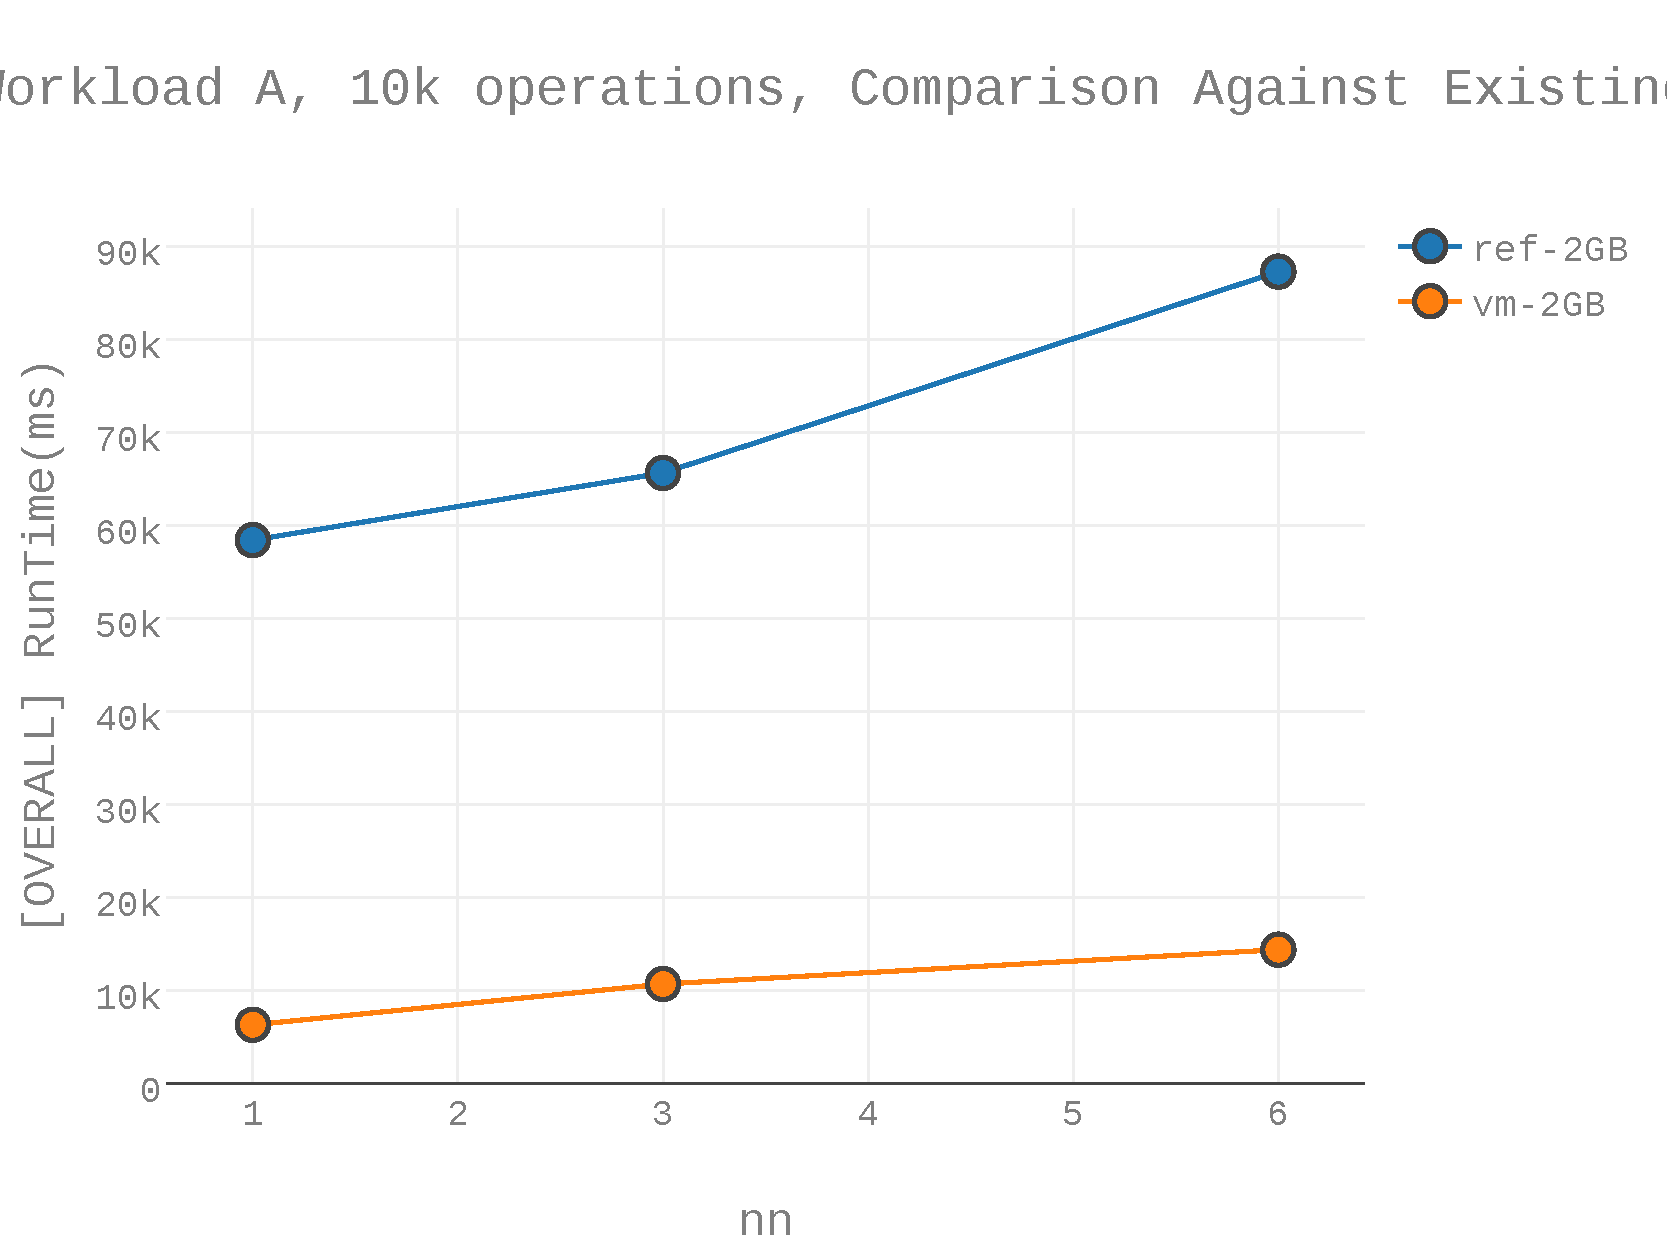
\includegraphics[width=6in]{Figures/figures-wla_fig5.pdf}

\caption{Comparing the results in \cite{Abramova2014} with the median value of the virtual machine assigned 2GB of \gls{ram}.  Note that the virtual machines were on a nodal network (minimal propagation delay) while the the links in \cite{Abramova2014} were unspecified.}

\label{fig:figures-wla_fig5}
\end{figure}

The summary for the 2GB-\gls{ram} virtual node are in Tables \ref{table:summary_statistics_for_1_config}, \ref{table:summary_statistics_for_3_config}, and \ref{table:summary_statistics_for_6_config} under column 'ram2GB'.    Figure \ref{fig:figures-wla_fig5} compares the results from \cite{Abramova2014} and the median execution times on a virtual machine environment for 1, 3, and 6 node configurations.  One can see a stark contrast between the execution times.

The most significant controlled difference between these two setups is the network.  The network in \cite{Abramova2014} is not specified, but generally a 'cluster' implies some kind of Ethernet configuration.  In a sense, this gives some insight into what kind of penalty one pays for switching from an ideal network to a physical one.

For the cluster sizes queried for this graph, both the virtual machine environment and the analagous workload done in \cite{Abramova2014} seem to positively correlate with cluster size.  This seems to indicate that, to a limited extent, the operations needed to ensure replication on multiple nodes overwhelm any advantage that dividing such operations among nodes.

One would expect, given that once this is extended to the Raspberry Pi modules, implying a physical network connection (Ethernet) and a 900 MHz processor compared to the 2.90 GHz processor used by the virtual machines, the performance would be represented by significantly longer execution time than that of the virtual nodes, possibly execution time comparable to the results in \cite{Abramova2014}.

Facing minimal propagation delay due to being connected on a nodal network and the same computing power as a laptop, in this work, results from the virtual machines seek to illustrate an asymptote on potential \gls{iot} performance expectations.

\section{Testing various memory sizes}

We now discuss testing and performance for memory sizes ranging from 512MB to 4GB.

\subsection{Minimum capability - 512MB}

This author reached a limit when attempting to examine operation with 512 MB of \gls{ram}.  Upon executing Cassandra, the program reported a deficiency in memory in order to operate.  This indicates that Cassandra has a minimum \gls{ram} capability to operate, although it is out of scope of this work to determine what parameters describe that limit.  

This author was not able to find an explicit hardware requirement for Cassandra, although in \cite{CassandraHardwareWiki}, a recommendation of 4GB RAM can be found.  However, the work in \cite{Abramova2014} shows that 2GB RAM is enough to run Cassandra.  This seems to suggest that through the right configurations of Cassandra, or Java upon which Cassandra runs, Cassandra might be able to work on platforms that have less RAM available.  With respect to this work, though not every configuration option was exhausted, and this may be an avenue for future work.    

\subsection{Experimental Testing for Memory in the 1GB – 4GB Range}

This section describes the results of running the \gls{ycsb} on virtual node networks as described in the methodology.  The summary of execution times are reported in Tables \ref{table:summary_statistics_for_1_config}, \ref{table:summary_statistics_for_3_config}, and \ref{table:summary_statistics_for_6_config}.  For each table, the summary statistics are listed for each amount of memory.

\subsubsection{Inspection of Results}

It is best to start with a visual inspection of the data represented in Figure \ref{fig:figures-wla_fig4}.  Generally with a greater amount of \gls{ram}, one might expect a correlation of fewer problems with memory overloads, or a lower frequency of compaction. However, inspection of each cluster size does not seem to indicate a correlation between memory and performance.

\begin{figure}[h]
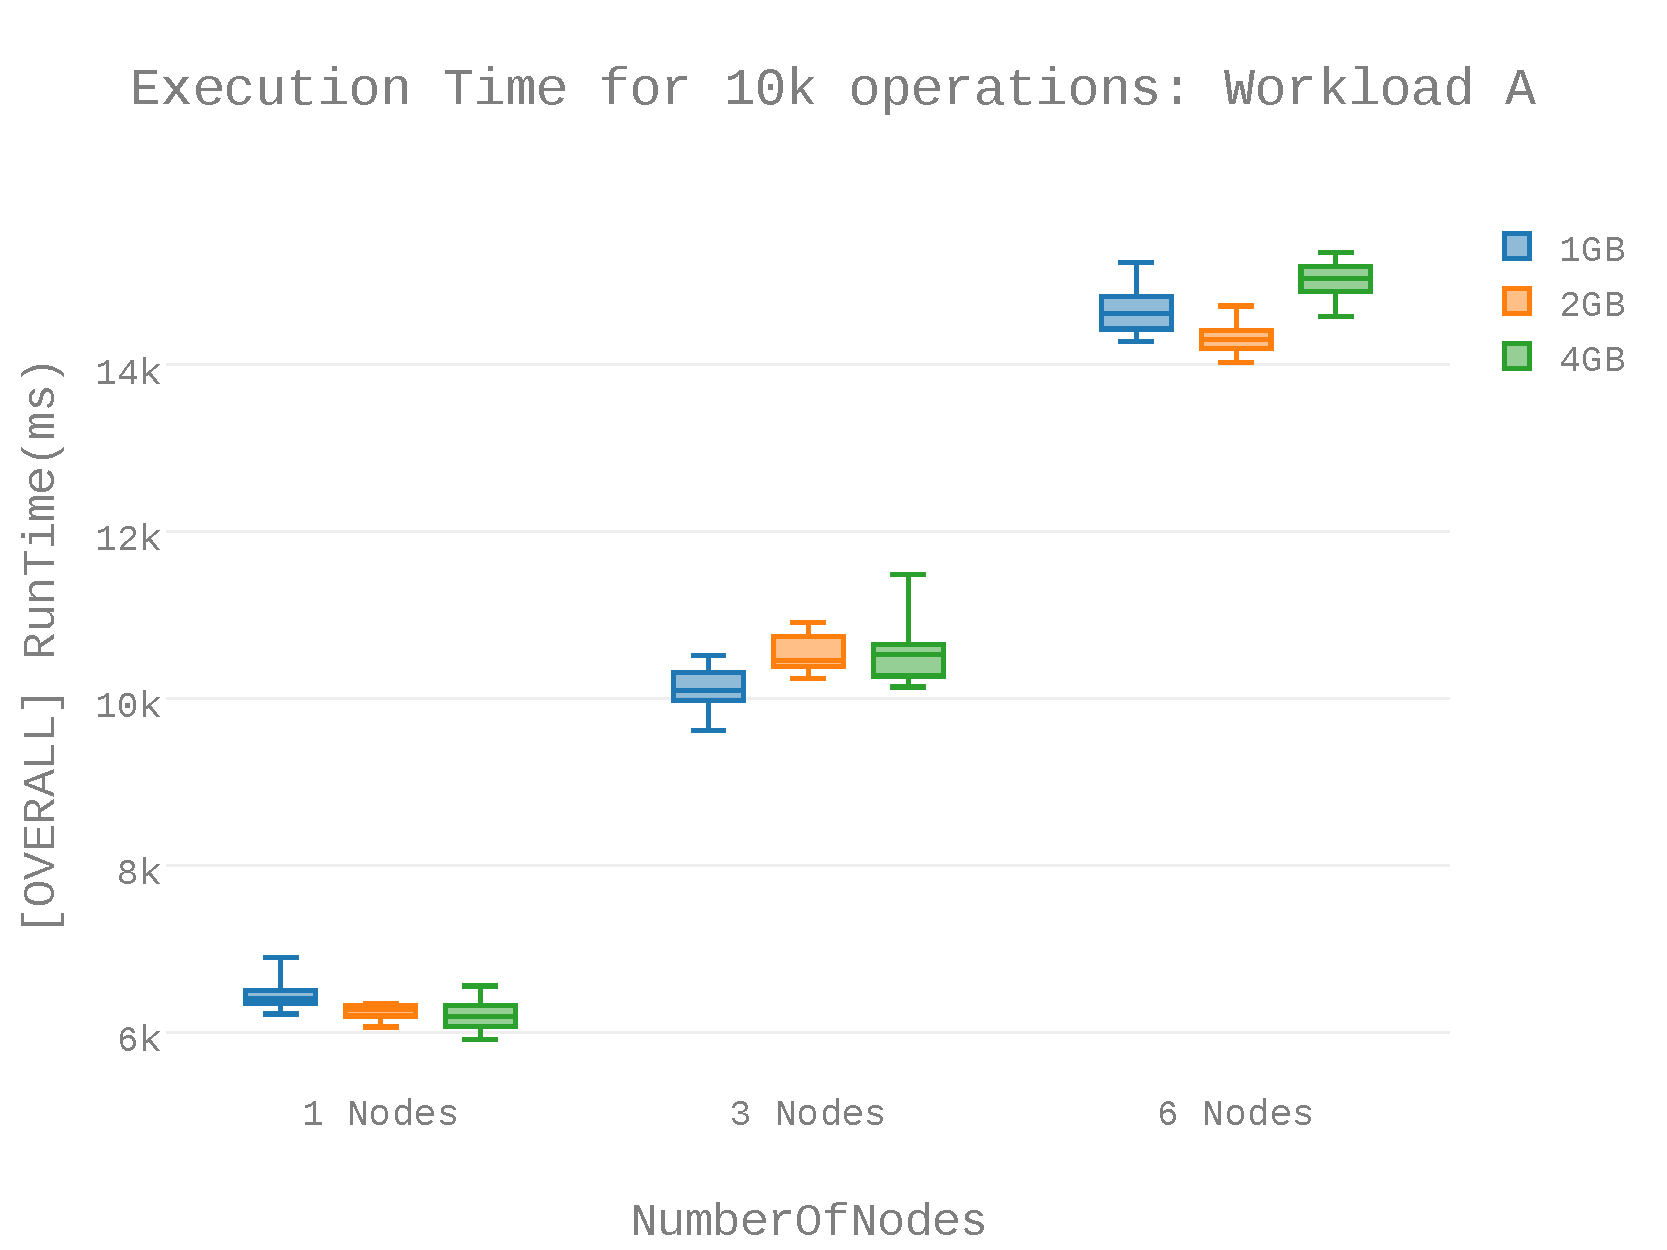
\includegraphics[width=3.5in]{Figures/figures-wla_fig4.pdf}

\caption{Execution time for virtual machines with 1GB, 2GB, and 4GB of \gls{ram}.  The first 9 trials have been removed in order to filter out the trials representing the cache effect and thus represent the steady state.}

\label{fig:figures-wla_fig4}
\end{figure}

\begin{table}
\begin{tabular}{lrrr}
\toprule
 index &  ram1GB &  ram2GB &  ram4GB \\
\midrule
 count &      21 &      21 &      21 \\
  mean & 6433.14 & 6246.24 & 6203.14 \\
   std & 144.084 & 84.0255 & 174.375 \\
   min &    6217 &    6062 &    5911 \\
   25\% &    6360 &    6207 &    6076 \\
   50\% &    6403 &    6278 &    6186 \\
   75\% &    6496 &    6318 &    6299 \\
   max &    6891 &    6345 &    6553 \\
 range &     674 &     283 &     642 \\
\bottomrule
\end{tabular}
\caption{Summary Statistics for 1-Node Configuration. All values represented fall between 5911.0 ms and 6891.0 ms, or rather within a span of 980.0 ms.}
\label{table:summary_statistics_for_1_config}
\end{table}

\begin{table}
\begin{tabular}{lrrr}
\toprule
 index &  ram1GB &  ram2GB &  ram4GB \\
\midrule
 count &      21 &      21 &      21 \\
  mean & 10127.9 & 10548.1 & 10549.1 \\
   std & 229.485 &  221.21 & 336.981 \\
   min &    9617 &   10235 &   10137 \\
   25\% &    9973 &   10382 &   10275 \\
   50\% &   10100 &   10456 &   10525 \\
   75\% &   10302 &   10735 &   10640 \\
   max &   10517 &   10910 &   11485 \\
 range &     900 &     675 &    1348 \\
\bottomrule
\end{tabular}
\caption{Summary Statistics for 3-Node Configuration. All values represented fall between 9617.0 ms and 11485.0 ms, or rather within a span of 1868.0 ms.}
\label{table:summary_statistics_for_3_config}
\end{table}

\begin{table}
\begin{tabular}{lrrr}
\toprule
 index &  ram1GB &  ram2GB &  ram4GB \\
\midrule
 count &      21 &      21 &      21 \\
  mean & 14659.3 & 14300.5 &   15000 \\
   std & 266.999 & 166.709 & 216.828 \\
   min &   14277 &   14030 &   14583 \\
   25\% &   14432 &   14200 &   14876 \\
   50\% &   14613 &   14298 &   15035 \\
   75\% &   14802 &   14407 &   15177 \\
   max &   15229 &   14705 &   15351 \\
 range &     952 &     675 &     768 \\
\bottomrule
\end{tabular}
\caption{Summary Statistics for 6-Node Configuration. All values represented fall between 14030.0 ms and 15351.0 ms, or rather within a span of 1321.0 ms.}
\label{table:summary_statistics_for_6_config}
\end{table}

\subsubsection{Absolute Ranges}

While Figure \ref{fig:figures-wla_fig4} gives a general sense of what the results look like, the actual summary statistics can be examined in Tables \ref{table:summary_statistics_for_1_config}, \ref{table:summary_statistics_for_3_config}, and \ref{table:summary_statistics_for_6_config}. After filtering out the first nine trials, the results for running 10,000 operations is displayed in Tables \ref{table:summary_statistics_for_1_config}, \ref{table:summary_statistics_for_3_config}, and \ref{table:summary_statistics_for_6_config}.  For each configuration, varying the \gls{ram} of the virtual machine resulted in execution times that fell within 2 seconds of each other.

\subsubsection{\gls{anova}}

A one-way \gls{anova} was performed with the filtered data, and the \gls{anova} summary tables can be seen in Tables \ref{ram_variance_analysis_workload_a_1_node}, \ref{ram_variance_analysis_workload_a_3_node}, and \ref{ram_variance_analysis_workload_a_6_node} for the 1, 3, and 6 node cases respectively.  For each case, the  p-value is much, much less than 0.05, and thus it can be said that one can be 95\% confident in the decision to fail to reject the null hypothesis that the means are equal.

\begin{table}
\begin{tabular}{lrrrrr}
\toprule
         Source &      SS &  df &      MS &   F &       p \\
\midrule
 between groups & 6.3e+05 &   2 & 3.1e+05 &  16 & 2.4e-06 \\
  within groups & 1.2e+06 &  60 & 1.9e+04 & nan &     nan \\
          total & 1.8e+06 &  62 &     nan & nan &     nan \\
\bottomrule
\end{tabular}
\caption{ANOVA Summary Table for Workload A, 1 Node}
\label{ram_variance_analysis_workload_a_1_node}
\end{table}

\begin{table}
\begin{tabular}{lrrrrr}
\toprule
         Source &      SS &  df &      MS &   F &       p \\
\midrule
 between groups & 2.5e+06 &   2 & 1.2e+06 &  17 & 1.2e-06 \\
  within groups & 4.3e+06 &  60 & 7.2e+04 & nan &     nan \\
          total & 6.8e+06 &  62 &     nan & nan &     nan \\
\bottomrule
\end{tabular}
\caption{ANOVA Summary Table for Workload A, 3 Node}
\label{ram_variance_analysis_workload_a_3_node}
\end{table}

\begin{table}
\begin{tabular}{lrrrrr}
\toprule
         Source &      SS &  df &      MS &   F &     p \\
\midrule
 between groups & 5.1e+06 &   2 & 2.6e+06 &  53 & 6e-14 \\
  within groups & 2.9e+06 &  60 & 4.9e+04 & nan &   nan \\
          total & 8.1e+06 &  62 &     nan & nan &   nan \\
\bottomrule
\end{tabular}
\caption{ANOVA Summary Table for Workload A, 6 Node}
\label{ram_variance_analysis_workload_a_6_node}
\end{table}

Examining the effects of variance in the amount of \gls{ram} allocated the virtual machines does not seem to have a notable impact on performance.  This indicates that, any observed limitation on the Raspberry Pis’ performance is not limited by \gls{ram}, but something else, and that varying \gls{ram} in future tests will not yield significant results.

% Insert something about statistical significance

\section{Implementation on Raspberry Pi}

In a similar fashion, the tests were run on the Raspberry Pi to observe performance.  The spread of each of the tests can be seen in Figure \ref{fig:wla_fig10} and Table \ref{table:wired-results}.  The results, next to one trend for the virtual machines, can be seen in Figure \ref{fig:fig06}. 

\begin{figure}[h]
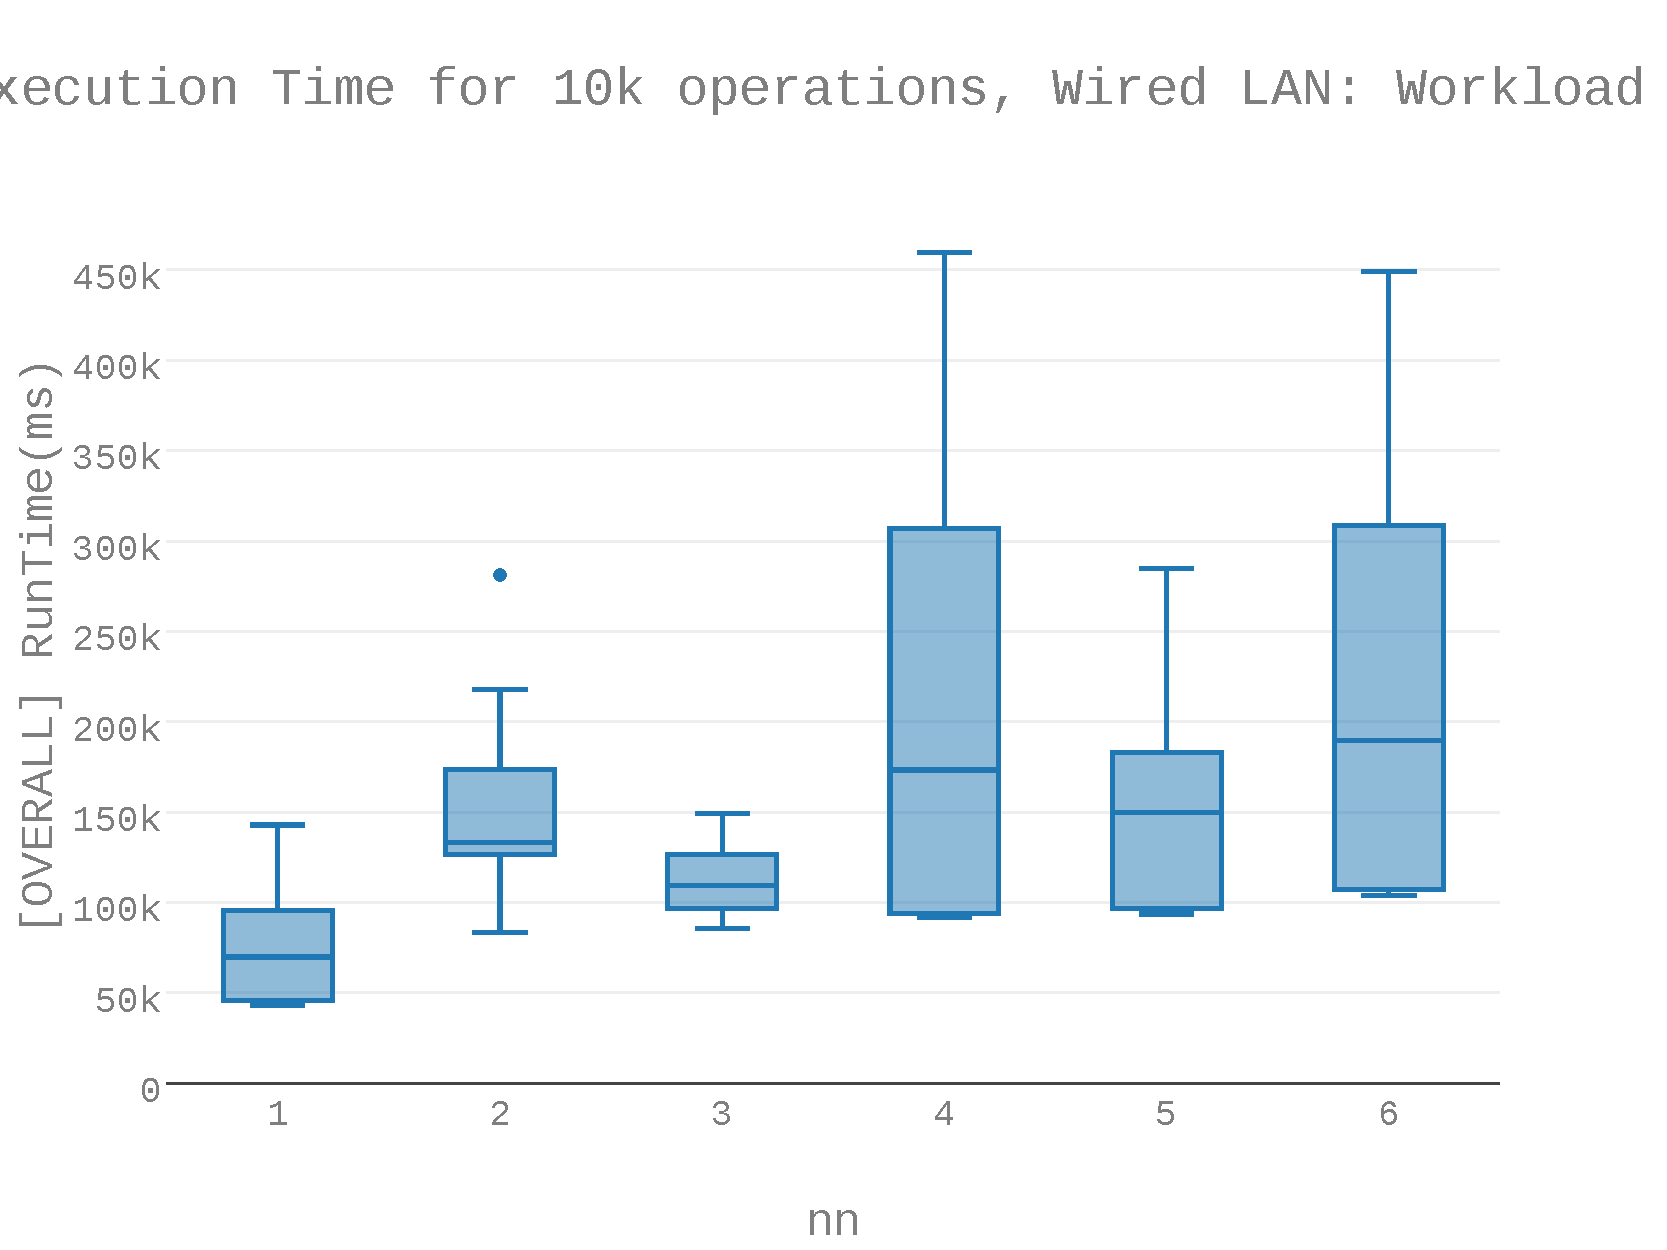
\includegraphics[width=3.5in]{Figures/figures-wla_fig10.pdf}

\caption{Box plot representing the results of the workload applied to wired local area network on the Raspberry Pi platform.}

\label{fig:wla_fig10}
\end{figure}

\begin{figure}[h]
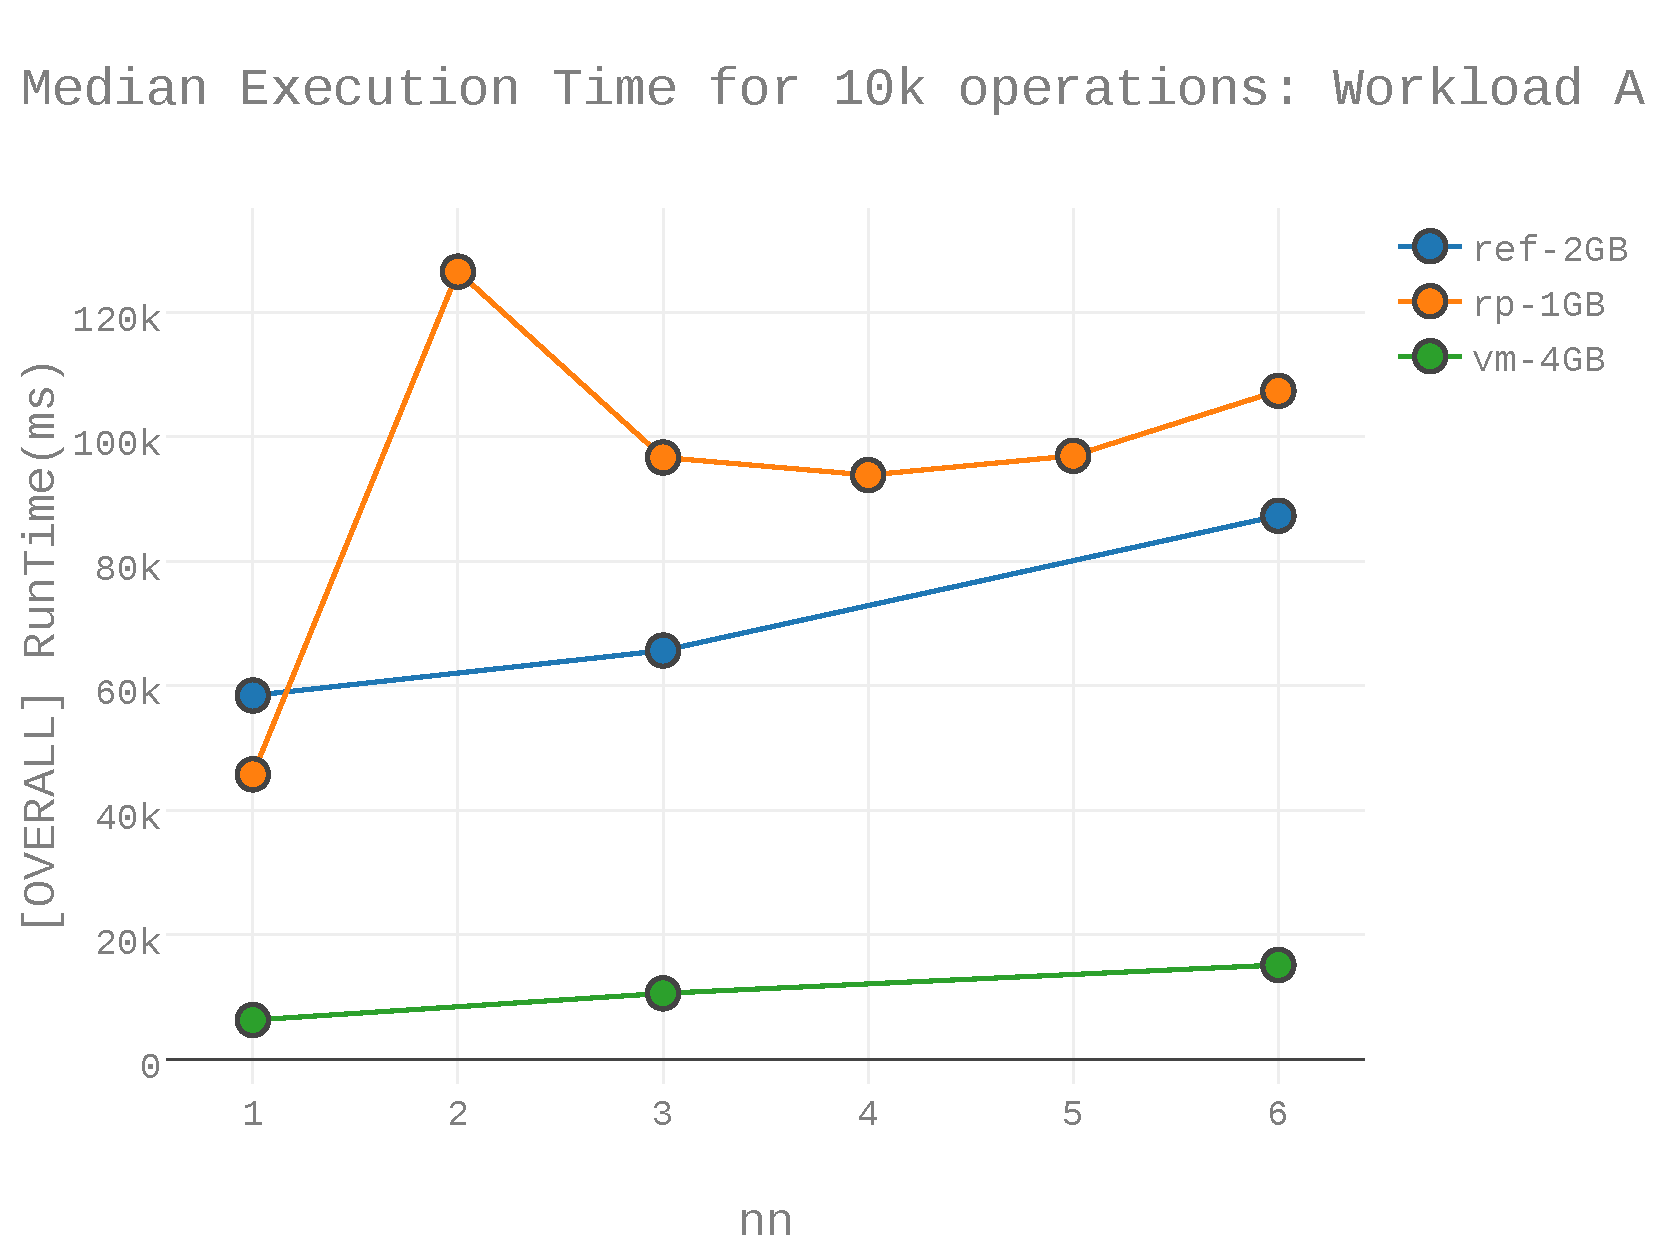
\includegraphics[width=3.5in]{Figures/figures-wla_fig6.pdf}

\caption{Comparison between the Raspberry Pi nodes (rp-1GB), the results reported in \cite{Abramova2014} (ref-2GB), and the virtual nodes with 4GB available \gls{ram} (vm-4GB).}

\label{fig:fig06}
\end{figure}

\begin{table}
\begin{tabular}{lrrr}
\toprule
 index &       1 &       3 &       6 \\
\midrule
 count &      21 &      21 &      21 \\
  mean & 4.6e+04 & 9.7e+04 & 1.1e+05 \\
   std & 1.1e+03 & 1.6e+03 & 1.8e+03 \\
   min & 4.3e+04 & 9.4e+04 &   1e+05 \\
   25\% & 4.5e+04 & 9.6e+04 & 1.1e+05 \\
   50\% & 4.6e+04 & 9.7e+04 & 1.1e+05 \\
   75\% & 4.6e+04 & 9.8e+04 & 1.1e+05 \\
   max & 4.8e+04 &   1e+05 & 1.1e+05 \\
 range & 4.9e+03 & 6.8e+03 & 7.3e+03 \\
\bottomrule
\end{tabular}
\caption{Summary for Raspberry Pi wired local area network}
\label{table:wired-results}
\end{table}

As can be seen from Figure \ref{fig:fig06}, the Raspberry Pi configuration takes considerably more execution time than the virtual machine analogy, which is probably due to the physical nature of the Ethernet connections (propagation delay) and the I/O limitations of the Raspberry Pi hardware.  However, its seemingly similar performance to the reference in \cite{Abramova2014} suggests the \gls{io} for the \gls{sd} Card follows a predictable pattern, and actually seems to outperform the node in \cite{Abramova2014} in the degenerate 1-node case.

For this paragraph, consider the results from \cite{Abramova2014} as the reference.  For a node network of 1, the experimental values fell between 43260.0 ms and 48123.0 ms, inclusive, and all values fell within 15170.0 ms of the reference value of 58430 ms.  For a node network of 3, the experimental values fell between 93702.0 ms and 100501.0 ms, inclusive, and all values fell within 34851.0 ms of the reference value of 65650 ms.  For a node network of 6, the experimental values fell between 103728.0 ms and 111002.0 ms, inclusive, and all values fell within 23692.0 ms of the reference value of 87310 ms.  

\section{Wireless Links}

The median value of the corresponding wired experiment will serve as the reference in this paragraph. For a node network of 1, the experimental values fell between 74072.0 ms and 119580.0 ms, inclusive, and all values fell within 73961.0 ms of the reference value of 45619.0 ms.  For a node network of 3, the experimental values fell between 123064.0 ms and 149252.0 ms, inclusive, and all values fell within 52156.0 ms of the reference value of 97096.0 ms.  For a node network of 6, the experimental values fell between 246945.0 ms and 355538.0 ms, inclusive, and all values fell within 248820.0 ms of the reference value of 106718.0 ms.

\begin{figure}[h]
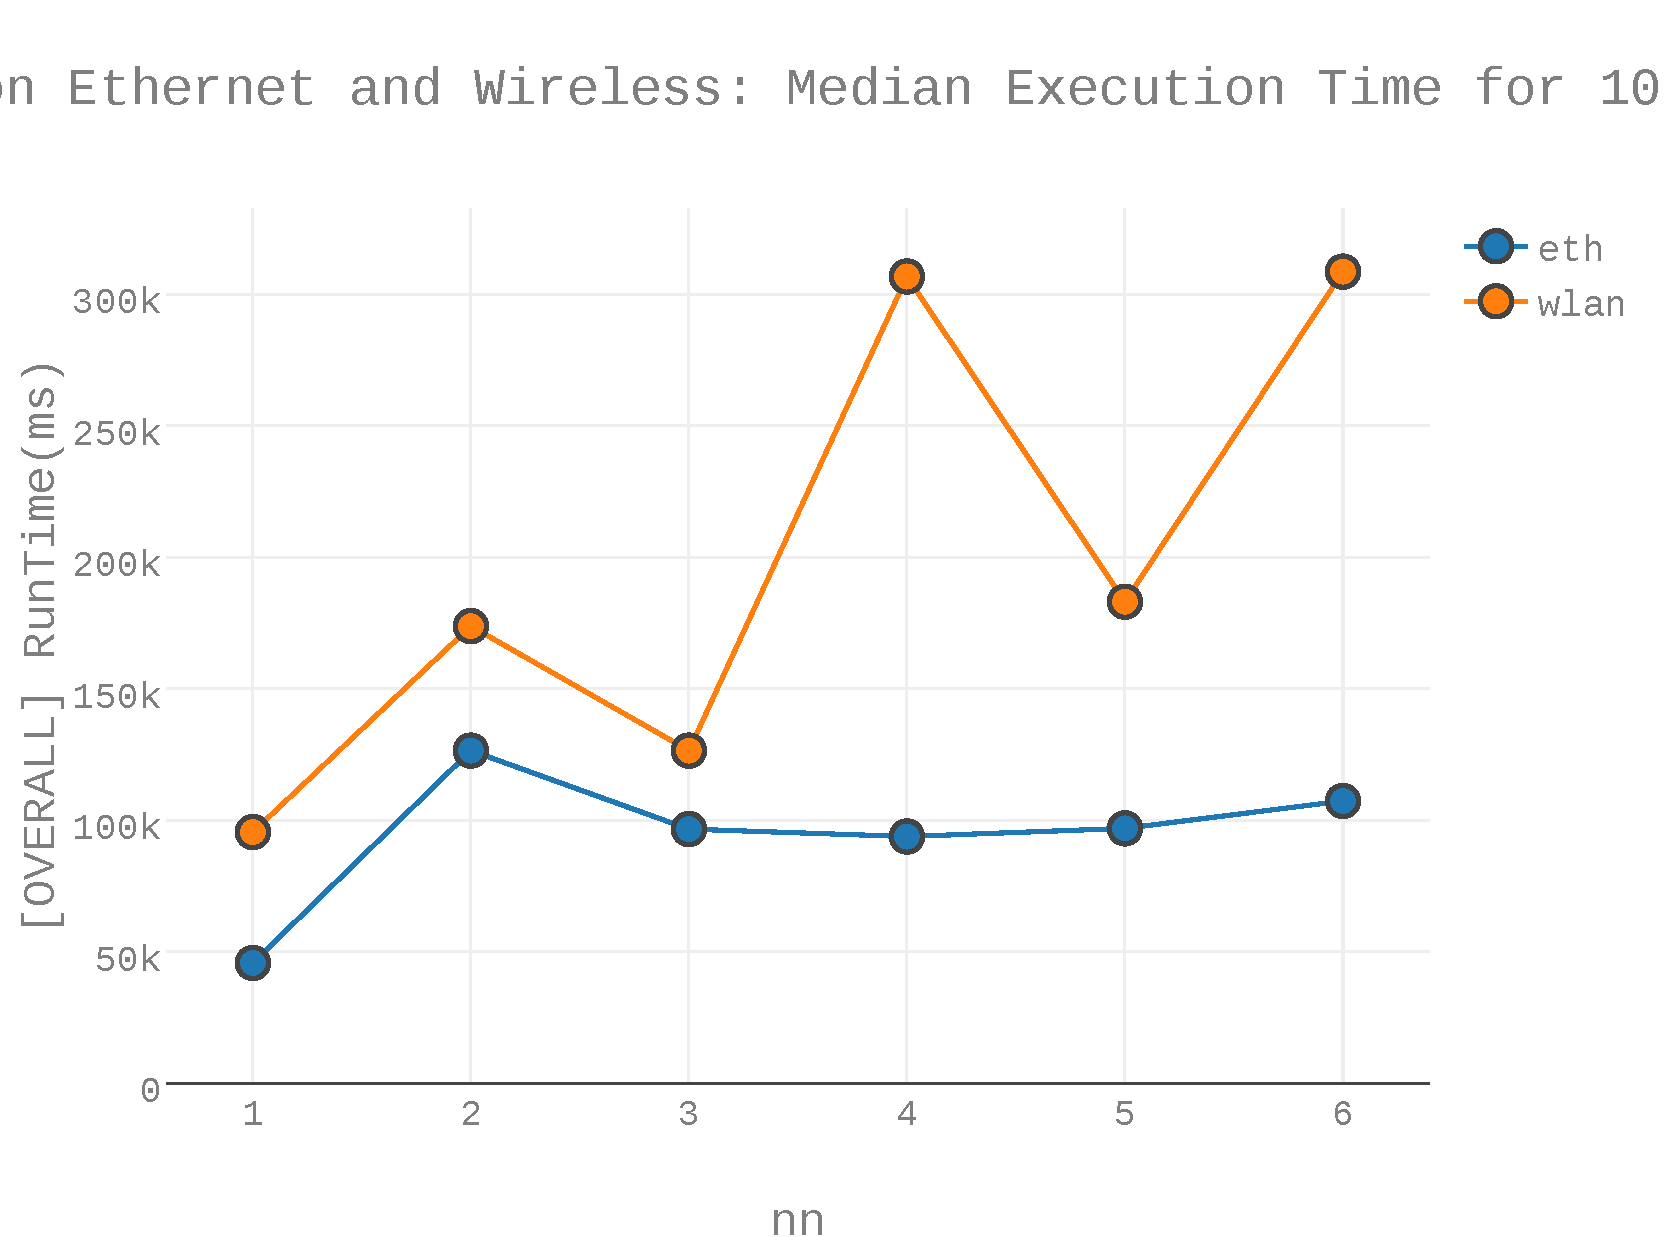
\includegraphics[width=3.5in]{Figures/figures-wla_fig7.pdf}

\caption{Comparison between the Ethernet links (eth) and wireless links (wlan) using the Raspberry Pi nodes.}

\label{fig:fig07}
\end{figure}

Figure \ref{fig:fig07} depicts the two experiments using Raspberry Pis: a wireless LAN (wlan) and an Ethernet LAN (eth).  In Figure \ref{fig:fig07}, as well as previous graphs, one can observe that the the Ethernet LAN effects about 50 seconds of execution time for 10,000 operations.  The initial median execution time for a node on a wireless LAN was found to be double the execution time.

For both configurations, performance takes a hit when transitioning from 1 to 2 nodes, but then increases from 2 nodes to 3 nodes.  From 3 nodes to 4 nodes, the wireless LAN configuration’s performance decreases dramatically, compared to slight increase in the wired Ethernet case.  

\begin{figure}[h]
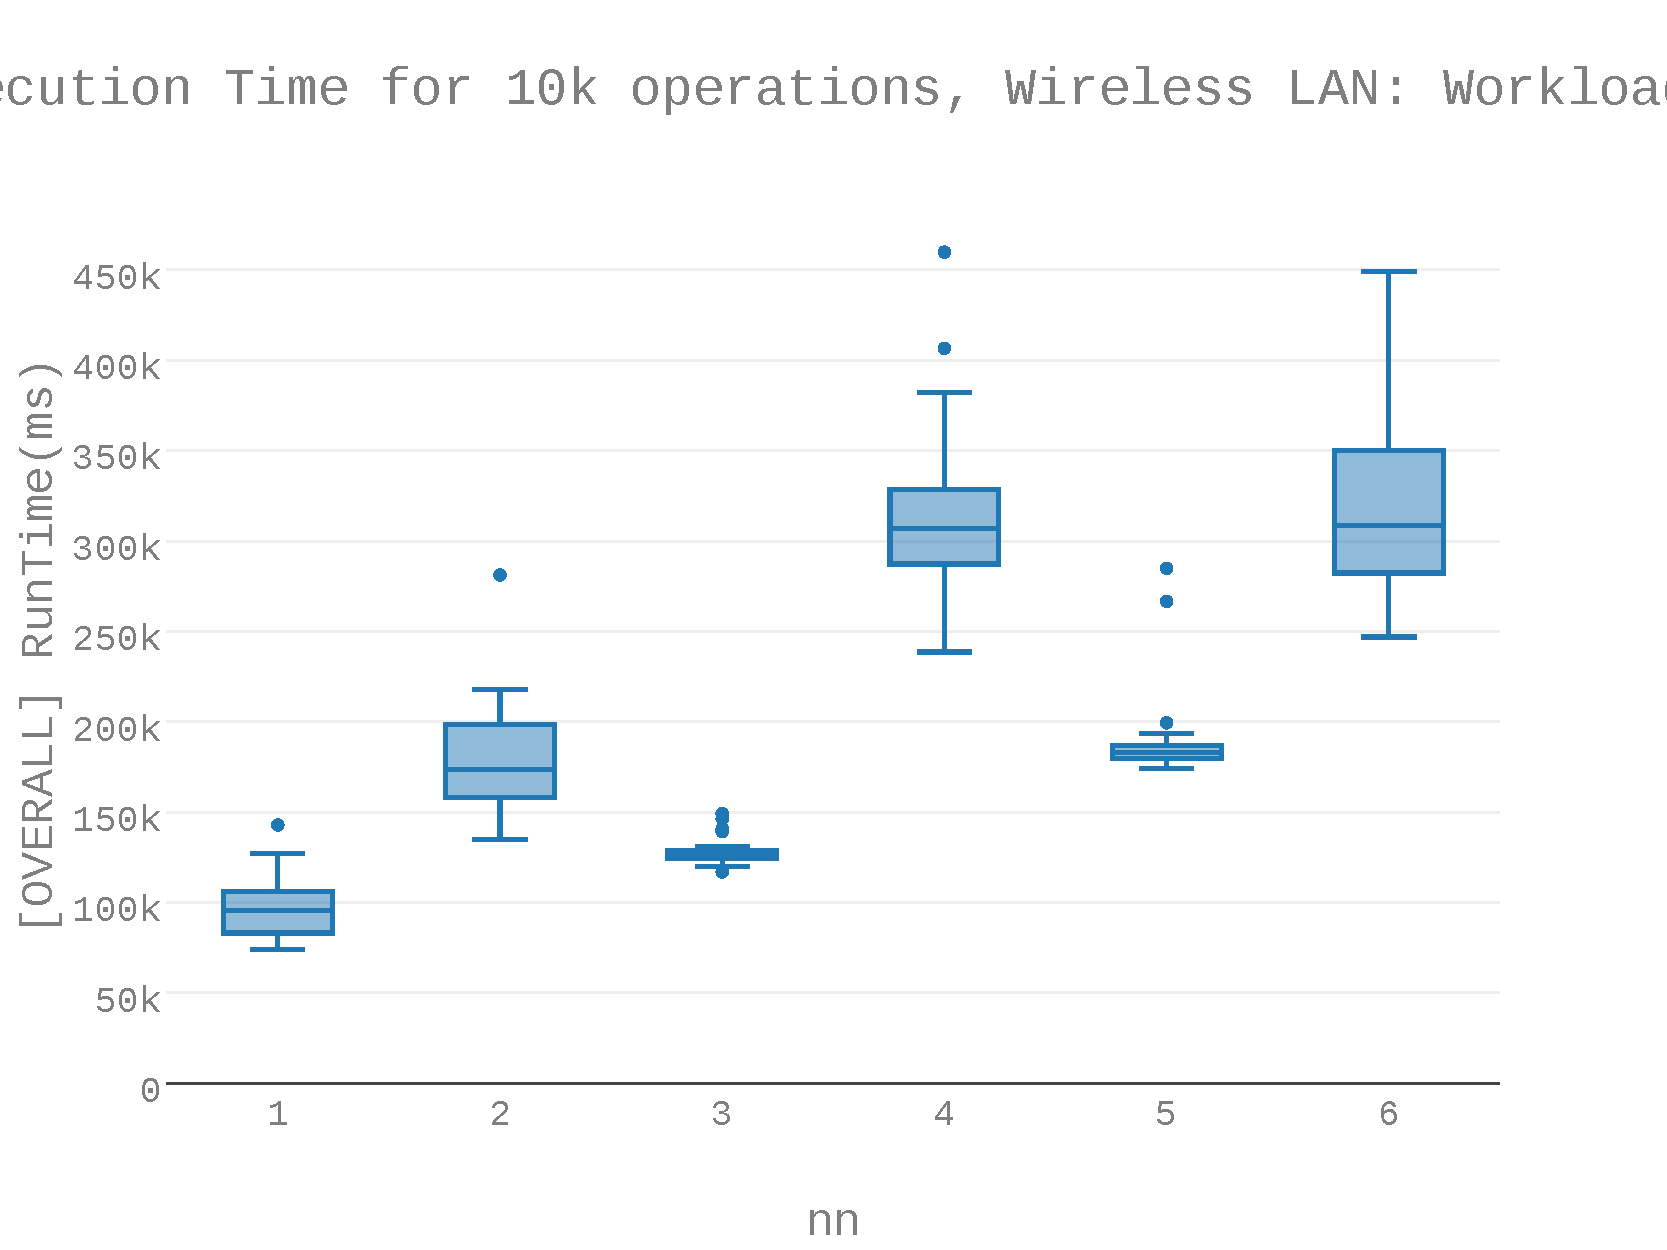
\includegraphics[width=3.5in]{Figures/figures-wla_fig8.pdf}

\caption{Distribution for all 30 trials of execution times where the Raspberry Pi nodes were connected via a wireless \gls{lan}.  Suspected outliers, values more than 3 times the interquartile range, are included as individual points above and below the 'maximum' and 'minimum' bars.}

\label{fig:fig08}
\end{figure}

A summary representation box plot of the results of wireless experimentation is above.  Here, the laptop was connected to the router via an Ethernet cable, and each node was connected to the router on a wireless local area network (LAN).  Suspected outliers, values more than 3 times the interquartile range (IQR) are included as points above and below.
There seems to be an overall increasing trend, while the data seems to oscillate, performing better for odd (1,3,5 node) configurations than for even (2,4,6 node) configurations.  However, there is no current theory behind this anomaly. 

\begin{figure}[h]
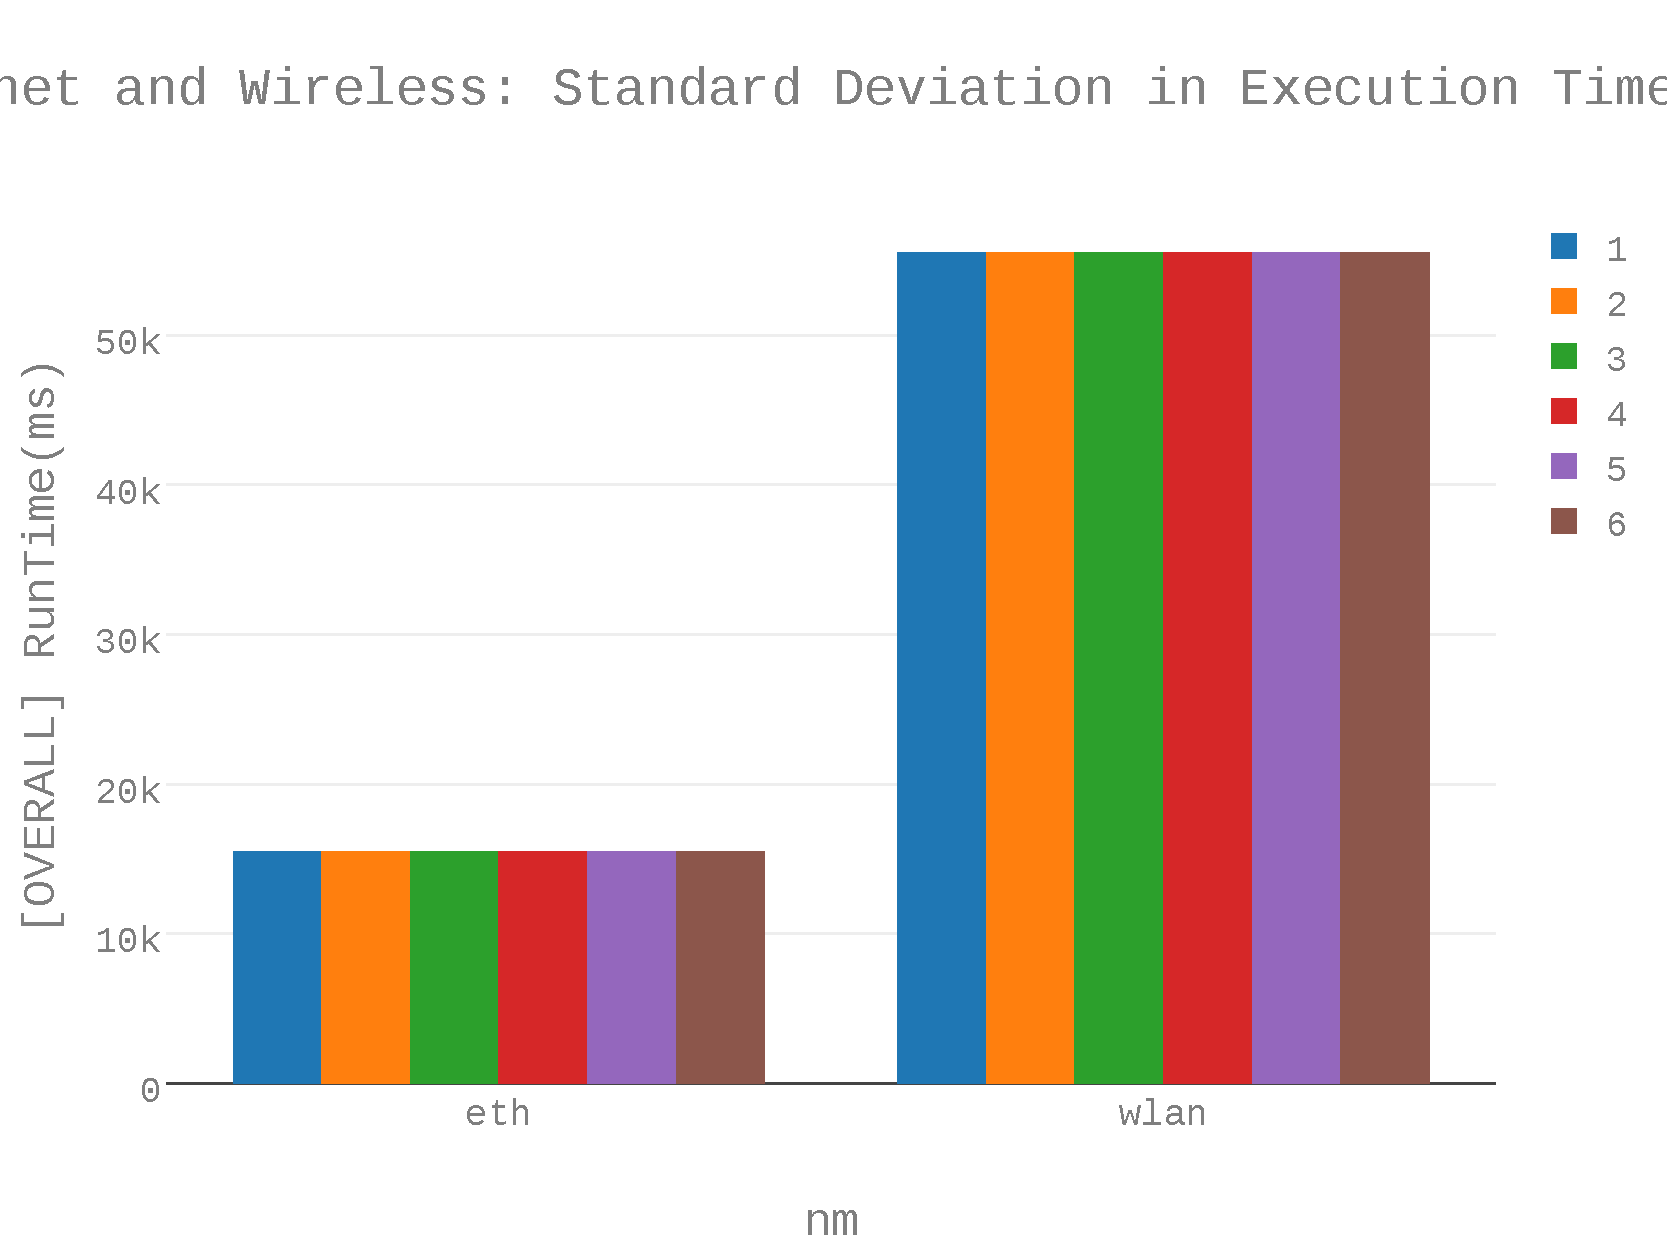
\includegraphics[width=3.5in]{Figures/figures-wla_fig9.pdf}

\caption{This compares the standard deviation in execution times for 10,000 operations of Workload A on the wired (eth) versus the wireless (wlan) configurations for 1 node, 2 nodes, 3 nodes, up through 6 nodes in milliseconds.}

\label{fig:fig09}
\end{figure}

To supplement the box plot, the standard deviation execution times for each set of trials, separated by number of nodes, is depicted in Figure \ref{fig:fig09}.  The difference seen here appears stark, and is overwhelming compared to the variance between 1, 2, 3, 4, 5 and 6 node networks given the same communication method. 

%1)      Reduced performance of Workload A is not statistically significant for the reduced memory sizes of IoT like devices
%2)      When varying platforms, performance for Workload A tracks the performance of the reference paper. For trials performe, reduced performance of Workload A is within 100ms of the reference paper (abramova) for wired implementations.
%3)      When varying communication method, reduced performance of Workload A is within 100ms of the wired platform test (order of magnitude, no greater than 100% increase in delay)
%4)      Reduced performance of Workload C is not statistically significant for the reduced memory sizes of IoT like devices
%5)      When varying platforms, reduced performance of Workload C is within 100ms of the reference paper (abramova) for wired implementations
%6)      When varying communication method, reduced performance of Workload C is within 100ms of the wired platform test
%7)      Reduced performance of Workload E is not statistically significant for the reduced memory sizes of IoT like devices
%8)      When varying platforms, reduced performance of Workload E is within 100ms of the reference paper (abramova) for wired implementations
%9)      When varying communication method, reduced performance of Workload E is within 100ms of the wired platform test
